%%%%%%
%
% $Autor: Sudeshna Nanda $
% $Datum: 2024-10-21 $
% $Pfad: ML23-06-Magic-Wand-with-an-Arduino-Nano-33-BLE-sense/manual/Contents/en/TechnicalSpecifications.tex $
% $Version: 1 $
%
%%%%%%



\chapter{Technical Specifications of Arduino Nano 33 BLE Sense and Other information}

\subsection{Specificatons}
{\begin{minipage}{\textwidth}
		\begin{center}
			\begin{tabular}{llm{100mm}} 
				\\ \textbf{\MapleCommand{Board Name}}  & Arduino® Nano 33 BLE Sense \\
				\textbf{\MapleCommand{Board SKU}}  & ABX00031\\
				\textbf{\MapleCommand{Microcontroller}}  & nRF52840\\
				\textbf{\MapleCommand{USB Connector}}  & Micro USB \\
				\textbf{\MapleCommand{Built-in LED Pin}}  & 13 \\
				\textbf{\MapleCommand{Digital I/O Pins}}  & 14 \\
				\textbf{\MapleCommand{Analog input pins}}  & 8 \\
				\textbf{\MapleCommand{PWM Pins}}  & 5\\
				\textbf{\MapleCommand{External Interrupts}}  & All digital pins\\
				\textbf{\MapleCommand{Bluetooth® Connectivity}}  & NINA-B306 \\
				\textbf{\MapleCommand{IMU(Accelerometer, Gyroscope, Magnetometer)}}  & LSM9DS1 \\
				\textbf{\MapleCommand{MICROPHONE}}  & MP34DT05 \\
				\textbf{\MapleCommand {GESTURE, LIGHT, PROXIMITY}}  & APDS9960 \\
				\textbf{\MapleCommand{BAROMETRIC PRESSURE}}  & LPS22HB \\
				\textbf{\MapleCommand{TEMPERATURE, HUMIDITY}}  & HTS221 \\	
				\textbf{\MapleCommand{UART}}  & RX/TX \\
				\textbf{\MapleCommand{I2C}}  & A4(SDA), A5(SCL)\\
				\textbf{\MapleCommand{SPI}}  & D11 (COPI), D12 (CIPO), D13 (SCK)\\ 
				&Use any GPIO for Chip Select (CS).\\
				\textbf{\MapleCommand{i/O Voltage}}  & 3.3V\\
				\textbf{\MapleCommand{Input Voltage (nominal)}}  & 5-18V \\
				\textbf{\MapleCommand{DC Current per I/O Pin}}  & 10 mA \\
				\textbf{\MapleCommand{Clock Speed Processor}} & 64MHz \\
				\textbf{\MapleCommand{CPU Flash Memory}}  & 1MB  \\
				\textbf{\MapleCommand{SRAM}}  & 256KB  \\
				\textbf{\MapleCommand{Weight}}  & 5 gr \\
				\textbf{\MapleCommand{Width}}  & 18mm \\
				\textbf{\MapleCommand{Length}}  & 45mm \\
			\end{tabular}
			\captionof{table}{Technical Specifications of Arduino Nano 33 BLE Sense \cite{Ard:2021}}
		\end{center}
\end{minipage}}

%\begin{figure}[h!]
	%\centering	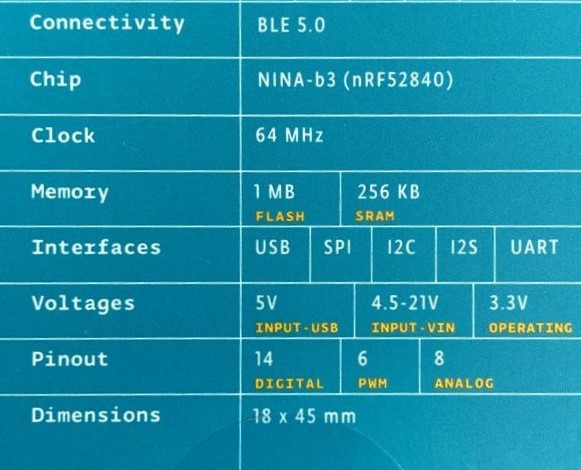
\includegraphics[width=9cm]{Images/spec}
	%\caption{\textbf{Technical Specification}}
%\end{figure}
\newpage

\subsection{Environmental Considerations}
\begin{itemize}
	\item This equipment complies with RF radiation exposure limits set forth for an uncontrolled environment.
	\item This Transmitter must not be co-located or operating in conjunction with any other antenna or transmitter.
	\item The operating temperature of the EUT can't exceed 85$^{0}$C and shouldn't be lower than -40$^{0}$C.
	\item The Frequency band should be in between 863-870Mhz.
	\item Arduino Nano 33 BLE only supports 3.3V I/Os and is NOT 5V tolerant so please make sure you are not directly connecting 5V signals to this board or it will be damaged.
	\item Keep away from water or fire.
	\item Hold it gently, do not harm the components and sensors present on the board.
\end{itemize}

\subsection{Extra Information}
\begin{enumerate}
	\item The design and specifications are subject to change without prior notice
	\item For information about the power supply, and more information about power consumption, refer
	to the label-rating attached to the product.
	\item Typical power consumption is measured according to international standard
\end{enumerate}

\subsection{Recommendation - EU Only}
This equipment may be used in both indoors and outdoors.
This equipment may be operated in all EU countries.
